\section{任务与方法}
\label{sec:framework}
\label{sec:framework:problem}

图修复需要两个相连的步骤：找到问题，再选择修改。我们连接图检查模块与修复模块。检查模块根据图和源文本构建评估概况。修复模块利用这一概况提出修改，并检查输出。

输入包括三元组列表 $G$、源文本 $X$、固定文档编号 $h_0$ 和允许关系 $\mathcal R_X$。列表可以包含同一三元组的多个副本。每种关系最多对应一个非空值，例如文档字段和收据字段。评分器用参考图 $G^*$ 检查输出。修复后的图记为 $\widehat G$。

主修复路径先清理输入，再让模型生成完整图，最后过滤三元组。错误报告或来源行提示可以引导生成。过滤器根据源文本和字段规则检查每个值。第二条路径利用尺度感知路由，每次选择一项编辑。它为试改后的图打分，并执行最佳允许编辑。第~\ref{sec:implementation}~节介绍两条路径及其测试设置。

\subsection{输入清理与错误报告}
\label{sec:framework:profile}

不同错误需要不同检查。重复三元组属于局部错误。错误的文档编号或字段名违反图规则。未在来源中出现的值无法通过证据检查。我们按实体、图和上下文三个范围组织检查。这里的上下文指文档源文本。图~\ref{fig:scale_relationship}~展示这三类检查。

\begin{figure}[t]
    \centering
    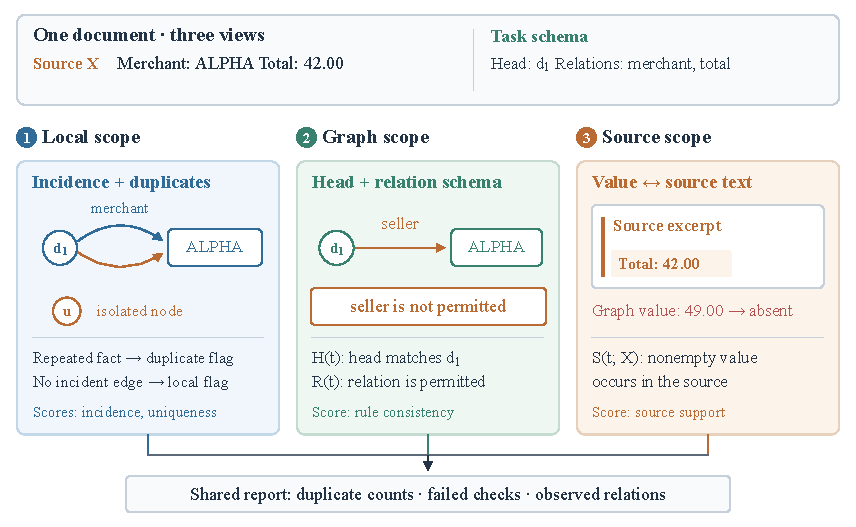
\includegraphics[width=0.98\textwidth]{figure/method/image2.pdf}
    \caption{图检查的三个范围。局部检查查找重复事实和无连接节点，图检查测试文档编号和字段名，来源检查在文本中查找值。两条修复路径都用这些检查构建评估概况。}
    \label{fig:scale_relationship}
\end{figure}

清理首先用明确的规则修正错误。预处理器 $P$ 删除重复三元组。若一条边的对象为 $h_0$，而主体是其他节点，则将该边反向。随后删除头节点或关系不合法的三元组。这里，头节点就是三元组的主体。清理后的图为 $G_s=P(G;h_0,\mathcal R_X)$。

对三元组 $t=(h,r,o)$，三项检查为
\begin{equation}
    \label{eq:diagnostic_predicates}
    H(t)=\mathbf1[h=h_0],\quad
    R(t)=\mathbf1[r\in\mathcal R_X],\quad
    S(t;X)=\mathbf1[o\ne\emptyset\ \wedge\ o\text{ 出现在 }X].
\end{equation}
$H$ 检查文档编号，$R$ 检查关系，$S$ 检查来源。分开执行这些检查，可以说明每条三元组被拒绝的原因。

主路径以错误报告的形式保存评估概况：
\begin{equation}
    \label{eq:diagnostic_context}
    D(G_s,X)=\big(n_{\mathrm{dup}},I_H,I_R,I_S,\mathcal R(G_s)\big).
\end{equation}
报告记录重复数、未通过检查的位置和已出现的关系。例如，$I_S=\{i:S(t_i;X)=0\}$ 列出未通过来源检查的位置。报告基于清理后的输入构建。它为模型提出字段值时提供查找位置。我们测试将报告加入提示的效果。字段为可选项，主路径对每篇文档调用模型一次。

\subsection{根据源文本生成图}
\label{sec:framework:architecture}

规则修正明确的结构错误；语言模型从文本中读取取值，并返回有序三元组列表：
\begin{equation}
    \label{eq:proposal_generation}
    C=L_\theta(X,h_0,\mathcal R_X,G_s,D(G_s,X)).
\end{equation}
提示要求模型生成完整图，复制来源值，保留正确字段，并补充或修正缺失、错误的值。JSON 解析器将无效响应记为空图。这些空图也计入评分。基础提示使用相同输入和输出上限，但去掉错误报告。

\subsection{检查生成的三元组}
\label{sec:framework:constraints}

约束决定哪些候选三元组进入修复后的图。门控是一个过滤器，在允许字段下保留与来源匹配的值，并保证每种关系最多有一个值。令 $\operatorname{uniq}(C)$ 按输出顺序去重。通过检查的三元组为
\begin{equation}
    \label{eq:eligible_candidates}
    C_X=\{t\in\operatorname{uniq}(C):H(t)R(t)S(t;X)=1\}.
\end{equation}
允许的输出集合为
\begin{equation}
    \label{eq:admissible_subsets}
    \mathcal F(C_X)=\left\{A\subseteq C_X:
    \sum_{t\in A}\mathbf1[r_t=r]\leq1,\ \forall r\in\mathcal R_X\right\}.
\end{equation}
式~\ref{eq:eligible_candidates}~规定证据和模式要求，式~\ref{eq:admissible_subsets}~规定字段数量上限。两者共同决定过滤器可以保留哪些输出。

过滤器按顺序扫描候选，保留每个字段的第一个有效值。输出 $\widehat G$ 的大小为
\begin{equation}
    \label{eq:selection_size}
    |\widehat G|=\max_{A\in\mathcal F(C_X)}|A|
    =|\{r:\exists t\in C_X,\ r_t=r\}|.
\end{equation}
每个字段构成一组，每组最多放一条三元组。只要该组中有有效候选，过滤器就保留其中一条。因此，它保留了允许范围内数量最多的候选。同一字段有多个值通过检查时，按输出顺序取舍。

\subsection{字段含义与来源行}
\label{sec:framework:field_evidence}

来源证据还帮助模型在相邻取值中作出选择。收据可能同时列出品牌、公司、小计和最终金额。我们为每个字段提供简短含义，引导模型选择。所有收据修复方法都获得这些字段含义和带行号的原文。

来源行索引为各字段增加提示。固定模式查找公司词、地址词、邮政编码、日期和总额标签。每条匹配行都是锚点。索引包含锚点行、前一行及后两行。简单流程 获得完整原文和字段含义。证据索引 还获得这些行提示。

收据过滤器与解析器使用相同空白规则。$N(s)$ 将连续空格或换行变成一个空格，并去掉首尾空白。来源检查为
\begin{equation}
    S_{\mathrm{ws}}(t;X)=\mathbf1[|N(o)|>0\ \wedge\
    N(o)\text{ 出现在 }N(X)].
\end{equation}
这一处理保留词边界、大小写和标点。收据后续测试使用该检查，早期测试使用原来的精确文本检查。

\section{实现}
\label{sec:implementation}

实现部分将检查转成修复步骤。第~\ref{sec:impl:assessment}~节介绍主生成与过滤路径。第~\ref{sec:impl:optimizer_audit}、\ref{sec:method:algorithm}~节介绍单独测试的编辑选择路径。

\subsection{修复步骤}
\label{sec:impl:assessment}

算法~\ref{alg:abstract}~给出 诊断＋门控。诊断 指错误报告，门控 指三元组过滤器。程序构建报告并执行检查，模型提出字段值，过滤器返回修复后的图和拒绝日志。

\begin{algorithm}[t]
\caption{利用源文本和字段检查进行修复}
\label{alg:abstract}
\begin{algorithmic}[1]
\Require 输入三元组 $G$、原文 $X$、文档编号 $h_0$、允许关系 $\mathcal R_X$
\Ensure 修复图 $\widehat G$ 和拒绝日志 $J$
\State $G_s\gets P(G;h_0,\mathcal R_X)$
\State $D\gets D(G_s,X)$
\State $C\gets\textsc{Parse}(L_\theta(X,h_0,\mathcal R_X,G_s,D))$
\State $\widehat G\gets\emptyset$; $J\gets\emptyset$; $B\gets\emptyset$
\For{按生成顺序遍历候选 $t=(h,r,o)$}
    \If{$t$ 之前已在 $C$ 中出现}
        \State 将 $(t,\text{重复})$ 加入 $J$
    \ElsIf{$H(t)R(t)S(t;X)=1$ 且 $r\notin B$}
        \State $\widehat G\gets\widehat G\cup\{t\}$; $B\gets B\cup\{r\}$
    \Else
        \State 将 $(t,\text{未通过检查})$ 加入 $J$
    \EndIf
\EndFor
\State \Return $\widehat G,J$
\end{algorithmic}
\end{algorithm}

运行程序将原文、文档编号、允许关系和输入三元组传给模型。评分器加载参考值。测试通过改变参考值和缺陷标签，确认模型输入保持一致。旧加载器从参考记录中读取文档编号，作为任务信息。

采用哈希查找时，清理平均需要 $O(|G|)$ 次三元组操作。过滤 $k$ 个候选的时间为 $O(k(1+c_X))$，额外内存为 $O(k+|\mathcal R_X|)$。这里，$c_X$ 表示在文本中查找一个值的成本，文本长度会影响这一成本。模型调用耗时与这些检查分别统计。

\subsection{提示与规则设置}
\label{sec:impl:enhancement}

\subsubsection{共享提示与响应}

同一个系统提示支持基础输入、错误报告和 SHACL 检查三种设置。每个输入调用三次，得到三个响应。每个响应在过滤前后分别计分，共得到六个分数。每个过滤前后对照使用相同三元组。这样，在衡量过滤器时，候选生成保持固定。

模型为 \texttt{google/gemma-4-26B-A4B-it}，温度为零。每种设置的输出上限均为 4,000 个 token。提示长度不同，因此我们报告输入 token 数。请求时间包含重试和请求间隔等待。所有响应均保存，无效响应也计分。较早的 Claude 测试为每种方法使用独立提示。

\subsubsection{SHACL 提示基线}
\label{sec:impl:shacl}

Lin 等人使用五部分提示：引言、检测到的错误、SHACL 规则、图上下文和指令\citep{ref_lin2025}。我们将其完整规则与完整图（$M+G$）设置用于字段任务。pySHACL 工具检查文档编号、允许关系、非空值和字段数量。SPARQL 规则根据原文检查取值。

提示包含完整原文，并返回完整 JSON 图。每篇文档的错误合并到一次调用中。我们将该基线称为\emph{Lin 风格 SHACL 上下文（改编版）}。RDF 保存唯一三元组，共享 JSON 输入保留重复副本。每种提示设置的输出都在过滤前后计分。

\subsection{尺度感知路由与编辑动作}
\label{sec:impl:optimizer_audit}
\label{sec:method:decision}

编辑选择器必须决定下一步修改图中的哪一部分。多项编辑可能针对同一字段，也可能撤销另一项编辑。选择器利用评估概况权衡这些选择。尺度感知路由为局部、图和来源编辑赋予权重。试改检查再比较各项收益与成本。图~\ref{fig:framework_overview}~展示这条路径。

\begin{figure}[t]
    \centering
    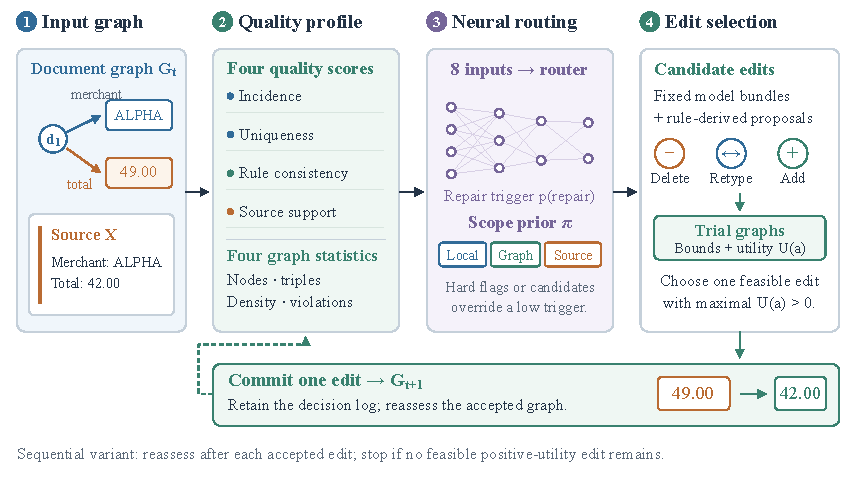
\includegraphics[width=0.98\textwidth]{figure/method/image1.pdf}
    \caption{用于编辑选择的尺度感知路由。评估概况和图统计量输入路由器，得到修复分数和三个编辑范围的权重。选择器在图副本上尝试模型与规则编辑，执行最佳允许正分编辑，再次检查。}
    \label{fig:framework_overview}
\end{figure}

\subsubsection{评估概况与共享输入}
\label{sec:impl:profile_revision}

选择器的评估概况使用四个分数，分别衡量节点连接、三元组唯一性、规则一致和来源支持：
\begin{equation}
\label{eq:quality_state}
\begin{split}
\mathbf{s}={}&(Q_{\mathrm{inc}},Q_{\mathrm{uniq}},Q_{\mathrm{rule}},Q_{\mathrm{src}}),\\
Q_i={}&100(1-r_i),\quad Q=\tfrac14\sum_i Q_i.
\end{split}
\end{equation}
每个 $r_i$ 是对应检查的错误率。对于非空图，各错误率为
\begin{equation}
\label{eq:profile_rates}
r_{\mathrm{inc}}=\frac{I}{n},\quad
r_{\mathrm{uniq}}=\frac{m-c}{m},\quad
r_{\mathrm{rule}}=\frac{B}{m},\quad
r_{\mathrm{src}}=\frac{V}{m}.
\end{equation}
$I$ 为无连接节点数，$c$ 为三元组相似组数。$B$ 为被图规则标记的不同三元组数。$V$ 为去掉空白后仍未在文本中出现的值的数量。这里，$n$、$m$ 分别为节点数和三元组数。这些分数为比较试改图提供统一尺度。空图的节点连接分为零，其余三项为 100。非空图没有源文本时，来源分为 50。

三元组相似度使用主体、关系和值的字符对计数。三部分余弦相似度的权重为 0.4、0.2、0.4。相似度达到 0.92 的三元组对组成相似组，用于唯一性评分。层级检查使用管理、监督和成员关系的方向，跳过含义不明确的关系。实体检查作用于标记为实体引用的端点，其他字段值按文本处理。

评估概况也报告来源字段缺失。来源字段检查读取文档、行或句子开头的允许标签之后的值。当原文给出一个字段而图中缺少它时，增加一个候选。重复标签给出冲突值时，跳过该字段。这些报告进入违规计数和候选列表。

路由器接收四项分数和四个图统计量：
\begin{equation}
\label{eq:routing_inputs}
\mathbf{g}=(n,m,\rho,n_{\mathrm{viol}}),\qquad
\rho=\frac{|E_{\mathrm{pair}}|}{n(n-1)}\quad(n>1).
\end{equation}
这里，$n$、$m$ 分别为节点数和三元组数。$E_{\mathrm{pair}}$ 包含不同的有向节点对，不含自连接。$n\leq1$ 时密度为零。$n_{\mathrm{viol}}$ 是报告的违规数。主报告 $D$ 列出字段错误，$\mathbf{s}$ 为选择器的图打分。两者都是评估概况，分别用于各自的修复路径。

\subsubsection{路由器与训练信号}

路由器将这八个输入转成修复分数和范围权重：
\begin{equation}
\label{eq:decision_net}
(p_{\mathrm{repair}},\boldsymbol{\pi})=
f_\phi(\operatorname{scale}([\mathbf{s};\mathbf{g}])).
\end{equation}
$\operatorname{scale}$ 使用训练集均值和标准差。$\boldsymbol{\pi}$ 有三个非负权重，合计为一，分别对应实体、图和上下文编辑。网络层大小为 $8\!\rightarrow\!32\!\rightarrow\!16$，具有一个修复输出和三个范围输出，共 884 个参数。两个隐藏层均使用 ReLU。sigmoid 给出修复分数，softmax 给出范围权重。训练和使用时共用特征代码。特征版本不匹配时，路由器改用等权重。

训练标签来自已知注入缺陷。损坏图的修复标签 $y_j$ 为一，其干净配对图的标签为零。范围标签 $c_j$ 取图中最常见的缺陷范围。干净图只训练修复输出。损失为
\begin{equation}
\label{eq:decision_loss}
\begin{split}
\mathcal L(\phi)={}&\frac1N\sum_j\operatorname{BCE}(p_j,y_j)\\
&+\frac{\sum_j b_j(-\log\pi_{j,c_j})}{\sum_j b_j+\epsilon}.
\end{split}
\end{equation}
有范围标签时，$b_j$ 为一；$\epsilon$ 避免除零。第一项训练修复分数，第二项用损坏图训练范围权重。同一文档组只属于训练、验证或测试中的一个划分。选择器根据任务输入和源文本计算特征。

\subsubsection{候选编辑与成本}
\label{sec:method:modalities}

规则和模型建议提供候选编辑。选择器可以删除三元组、改变关系或添加三元组。改变关系在代码中称为 retype。相关编辑可以组成一个包。在保存建议测试中，清理后输入与模型输出之间的差异按关系分组。每组是一个置信度为 0.7 的编辑包。

编辑成本鼓励小幅修改：
\begin{equation}
\label{eq:cost_hierarchy}
c(a)=\begin{cases}
0.30 & \text{删除},\\
0.16 & \text{改关系},\\
0.06 & \text{添加}.
\end{cases}
\end{equation}
编辑包的成本是其中各项编辑成本之和。这些固定成本与质量增益、范围权重一起进入试改分数。学习先验测试将路由器与始终开启的等权先验比较。

\subsection{试改检查与修复循环}
\label{sec:method:algorithm}

执行编辑前，先在图副本上试做每个候选。令 $G_a$ 为试改图，$h$ 为硬规则错误数，$\sigma(a)$ 为编辑范围，$z(a)$ 为候选置信度。默认分数为
\begin{equation}
\label{eq:action_utility}
\begin{split}
U(a)={}&\frac{Q(G_a)-Q(G)}{100}
+0.20\frac{\max(0,h(G)-h(G_a))}{\max(1,h(G))}\\
&-0.35c(a)+0.05\log\!\left(\max(\pi_{\sigma(a)},0.05)+10^{-6}\right)
+0.02z(a).
\end{split}
\end{equation}
各项分别衡量质量增益、规则错误减少、编辑成本、范围权重和候选置信度。试改重新计算完整图的评估概况，并检查分数边界、密度，以及编辑是否会把图删空。

四项分数的下界依次为 55、55、60、45。已经满足的下界必须继续满足。低于下界的分数必须保持或提高。在这些条件下，每项检查分数最多下降两分。试改后密度最多为 0.75，非空图必须保持非空。这些要求确定允许的试改集合 $\mathcal A_t^{\mathrm{ok}}$。选择步骤为
\begin{equation}
\label{eq:constrained_opt}
a_t^*=\arg\max_{a\in\mathcal A_t^{\mathrm{ok}}}U(a),\qquad U(a_t^*)>0.
\end{equation}
式~\ref{eq:constrained_opt}~在当前试改编辑中作出选择。边界决定哪些编辑允许执行，分数为允许编辑排序。没有允许编辑获得正分时，图保持原样。

\begin{figure}[t]
    \centering
    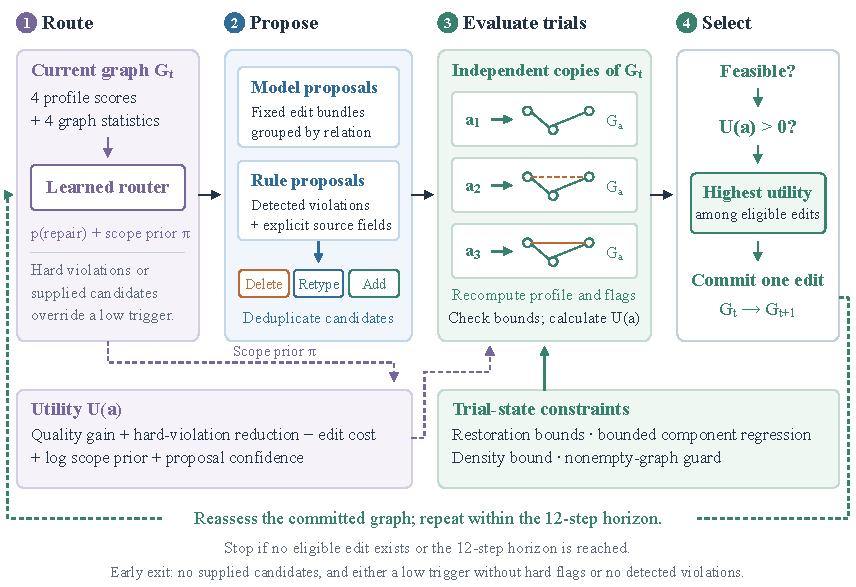
\includegraphics[width=0.98\textwidth]{figure/method/image3.pdf}
    \caption{一轮试改检查。路由器为编辑范围赋权，选择器在图副本上为每项模型或规则编辑打分、检查边界，并执行最佳允许正分编辑。随后重新构建评估概况。保存建议测试最多允许十二轮。}
    \label{fig:optimization_flow}
\end{figure}

算法~\ref{alg:enhancement}~连接评估、路由和执行。即使修复分数较低，只要存在已提供的候选或硬规则错误，也会开始试改检查。当没有有用的允许编辑、不再需要试改，或达到步数上限时，循环结束。日志保存试改图、分数、决策和停止原因。

\begin{algorithm}[t]
\caption{带试改检查的尺度感知编辑选择}
\label{alg:enhancement}
\begin{algorithmic}[1]
\Require 输入图 $G$、原文 $X$、已提供候选 $A_0$、任务输入、步数上限 $T$
\Ensure 修复图 $\widehat G$ 和决策日志 $J$
\State $\widehat G\gets G$; $J\gets\emptyset$; $E\gets\emptyset$
\State 将缺失来源字段的候选加入 $A_0$
\For{$t=1$ 到 $T$}
    \State 为 $\widehat G$ 计算评估概况和 $(p_{\mathrm{repair}},\boldsymbol\pi)$
    \If{$A_0=\emptyset$、$h(\widehat G)=0$ 且 $p_{\mathrm{repair}}<\tau_{\mathrm{repair}}$}
        \State \textbf{退出循环}
    \EndIf
    \If{没有报告的违规且 $A_0=\emptyset$}
        \State \textbf{退出循环}
    \EndIf
    \State $A\gets\textsc{Unique}(A_0\cup\textsc{RuleEdits}(\widehat G))$
    \State 跳过已在 $E$ 中的图与候选组合
    \State 对其余每个 $a\in A$ 在副本上试改，并将组合记入 $E$
    \State 为每次试改检查图边界并计算 $U(a)$
    \State 将试改分数和决策加入 $J$
    \If{没有允许候选满足 $U(a)>0$}
        \State \textbf{退出循环}
    \EndIf
    \State 对 $\widehat G$ 执行 $U(a)$ 最高的允许编辑
\EndFor
\State \Return $\widehat G,J$
\end{algorithmic}
\end{algorithm}

保存建议测试使用 $T=12$ 和 $\tau_{\mathrm{repair}}=0.05$。第二种评分从默认分数中减去 $0.05\log(1/3+10^{-6})$。这样，等权重的先验项为零。对于固定路由器，它保留编辑排序，但改变正分接受门槛。两种评分均在保存建议测试前固定。该选择器的来源匹配去掉两个字符串中的空白。档案也保留使用其他空白规则的早期日志。算法~\ref{alg:abstract}~和选择器分别测试。

对于 $m$ 条三元组，两两检查的成本为 $O(m^2)$。$T$ 轮、每轮最多 $K$ 次试改的成本为 $O(TKm^2)$，另加文本检查成本。主过滤器只扫描候选列表一次。